\section{后记}
容器类型是将模板引入C++编程语言的主要动机。模板之前,多态层次结构是容器的一种流行方法。一个例子是国立卫生研究院类库(NIHCL,National Institutes of Health Class Library),在很大程度上转换了Smalltalk容器类的体系(见图18.5)。

\begin{center}
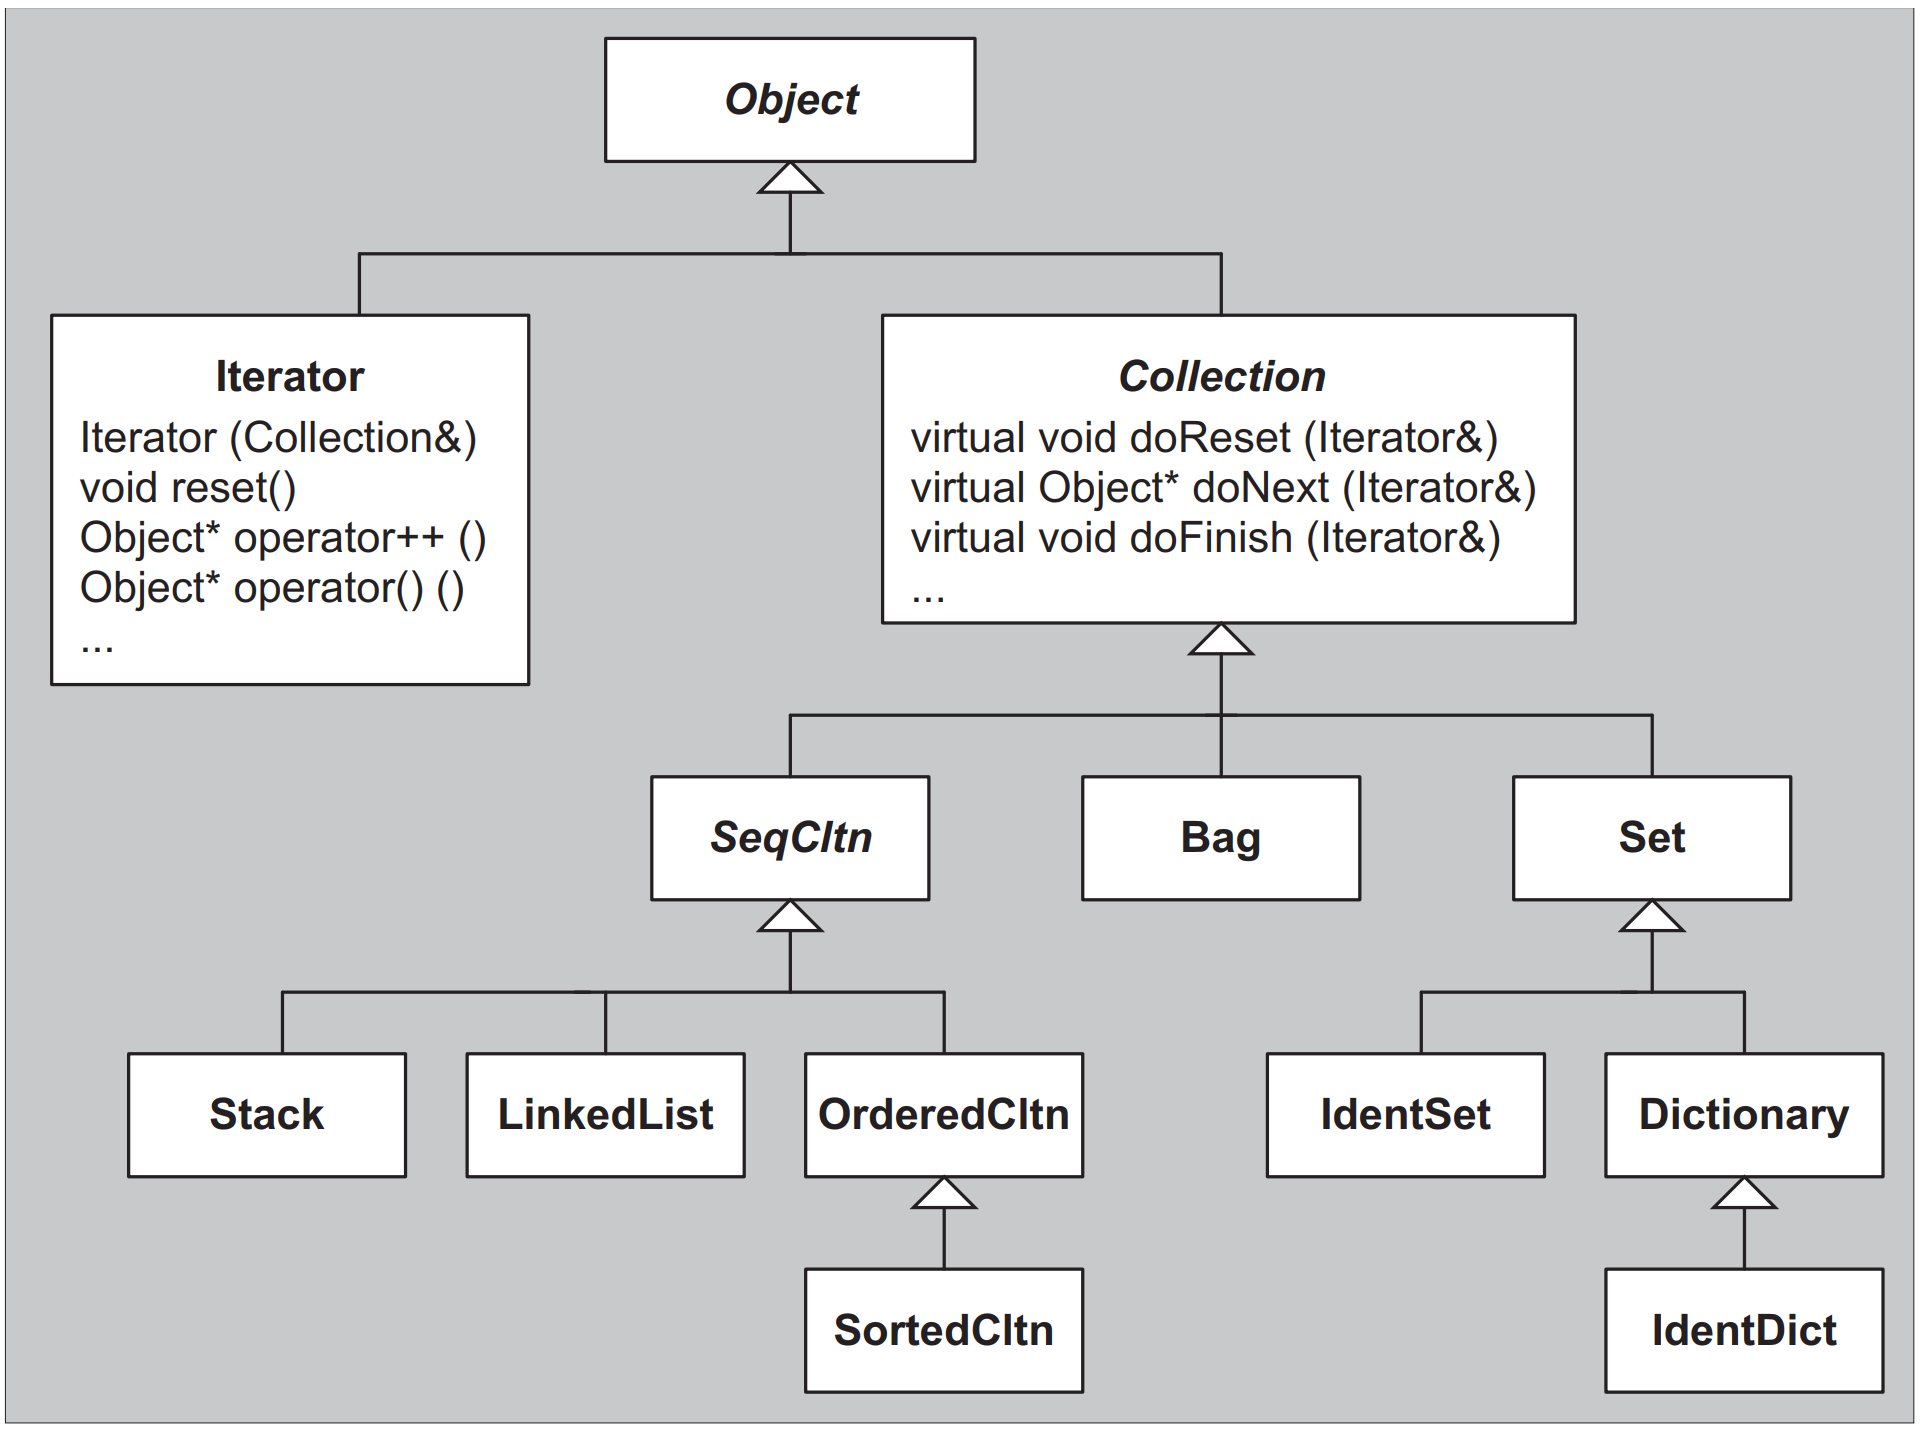
\includegraphics[width=0.8\textwidth]{part3/ch18/images/5.png} \\
图18.5. NIHCL的体系
\end{center}

与C++标准库类似,NIHCL支持丰富的容器和迭代器。但实现遵循了Smalltalk的动态多态风格:迭代器使用抽象基类Collection来操作不同类型的集合:

\begin{cpp}
Bag c1;
Set c2;
...
Iterator i1(c1);
Iterator i2(c2);
...
\end{cpp}

但就运行时间和内存用量而言,这种方法的代价很高。运行时间通常比使用C++标准库的等效代码差几个数量级,因为大多数操作最终都需要一个虚调用(而在C++标准库中,许多操作都是内联的,迭代器和容器接口中不涉及虚函数)。此外,由于(与Smalltalk不同)接口是有边界的,内置类型必须封装在更大的多态类中(这样的封装器由NIHCL提供),这反过来可能会导致存储需求的急剧增加。

即使在如今的模板时代,许多项目仍然在多态性的方法上做出次优选择。显然,动态多态性都是正确的选择,异构迭代就是一个例子。同样地,许多编程任务都可以使用模板有效地解决,同构容器就是一个例子。

静态多态可以很好地编写基本计算结构,而选择公共基类型的需要意味着动态多态库通常必须做出特定于领域的选择。因此,C++标准库的STL部分从未包含多态容器也不足为奇,但包含了一组使用静态多态的容器和迭代器(如第18.6节所示)。

中型和大型C++程序通常需要处理本章讨论的两种多态性。某些情况下,有必要将它们紧密地结合起来使用。根据我们的讨论,最优的设计选择很明确,花一些时间考虑长期的、潜在的回报是值得的。





















